\newpage
\section{Auswertung}

\subsection{Nullrate}

Die Nullrate $N_0$ wird als Mittelwert aus fünf Messungen, die je über $\increment=300\si{\second}$ durchgeführt wurden, bestimmt.\\
Bei den Messungen wurden, ohne jegliche zusätzliche Anregung des Zählrohrs, folgende Werte gemessen:
\begin{equation*}
    N_0 = \{129, 143, 144, 136, 139, 126, 158 \}
\end{equation*}
Gemittelt und auf $\increment=30\si{\second}$ normiert ergibt sich eine Zählrate von $N_0= 13.9286\si{\second}$, mit der auch im Folgenden gerechnet wird.\\


\subsection{Vanadium}

\begin{table}[!htbp]
    \centering
    \small
    \begin{tabular}{S [table-format=3.1] S [table-format=3.1] S [table-format=3.4] S [table-format=3.4]}
        \toprule
        {$t \mathbin{\scalebox{1.5} / }\si{\second}$} & {$N_V $} & {$N_V - N_0 $} & {$\sqrt{N_V - N_0 }$}\\
        \midrule
        30.0                 & 189.0                & 175.0714   & 13.231  \\
        60.0                 & 197.0                & 183.0714   & 13.530  \\
        90.0                 & 150.0                & 136.0714   & 11.664  \\
        120.0                & 159.0                & 145.0714   & 12.044  \\
        150.0                & 155.0                & 141.0714   & 11.877  \\
        180.0                & 132.0                & 118.0714   & 10.866  \\
        210.0                & 117.0                & 103.0714   & 10.152  \\
        240.0                & 107.0                & 93.0714   & 9.6473  \\
        270.0                & 94.0                 & 80.0714   & 8.9482  \\
        300.0                & 100.0                & 86.0714   & 9.2774  \\
        330.0                & 79.0                 & 65.0714   & 8.0666  \\
        360.0                & 69.0                 & 55.0714   & 7.4210  \\
        390.0                & 81.0                 & 67.0714   & 8.1897  \\
        420.0                & 46.0                 & 32.0714   & 5.6631  \\
        450.0                & 49.0                 & 35.0714   & 5.9221  \\
        480.0                & 61.0                 & 47.0714   & 6.8608  \\
        510.0                & 56.0                 & 42.0714   & 6.4862  \\
        540.0                & 40.0                 & 26.0714   & 5.1060  \\
        570.0                & 45.0                 & 31.0714   & 5.5741  \\
        600.0                & 32.0                 & 18.0714   & 4.2510  \\
        630.0                & 27.0                 & 13.0714   & 3.6154  \\
        660.0                & 43.0                 & 29.0714   & 5.3917  \\
        690.0                & 35.0                 & 21.0714   & 4.5903  \\
        720.0                & 19.0                 & 5.0714   & 2.2519  \\
        750.0                & 28.0                 & 14.0714   & 3.7511  \\
        780.0                & 27.0                 & 13.0714   & 3.6154  \\
        810.0                & 36.0                 & 22.0714   & 4.6980  \\
        840.0                & 25.0                 & 11.0714   & 3.3273  \\
        870.0                & 29.0                 & 15.0714   & 3.8821  \\
        900.0                & 18.0                 & 4.0714   & 2.0177  \\
        930.0                & 17.0                 & 3.0714   & 1.7525  \\
        960.0                & 24.0                 & 10.0714   & 3.1735  \\
        990.0                & 21.0                 & 7.0714   & 2.6592  \\
        1020.0               & 25.0                 & 11.0714   & 3.3273  \\
        1050.0               & 21.0                 & 7.0714   & 2.6592  \\
        1080.0               & 24.0                 & 10.0714   & 3.1735  \\
        1110.0               & 25.0                 & 11.0714   & 3.3273  \\
        1140.0               & 17.0                 & 3.0714   & 1.7525  \\
        1170.0               & 20.0                 & 6.0714   & 2.4640  \\
        1200.0               & 19.0                 & 5.0714   & 2.2519  \\
        1230.0               & 20.0                 & 6.0714   & 2.4640  \\
        1260.0               & 18.0                 & 4.0714   & 2.0177  \\
        1290.0               & 16.0                 & 2.0714   & 1.4392  \\
        1320.0               & 17.0                 & 3.0714   & 1.7525  \\
        \bottomrule
    \end{tabular}
\caption{Die Messwerte der Zerfallraten für Vanadium mit ihren korrespondierenden Zeiten. Zusätzlich auch noch ihr $\sqrt{N}$ Fehler und die Raten abzüglich Nullraten.}
\label{tab:Va}
\end{table}
\noindent
Für das Vanadium Isotop $\ce{^{52}_{}V}$ ergeben sich die in Tab.\ref{tab:Va} dargestellten Messwerte inklusive ihrer $\sqrt{N}$ Fehler.\\
Auf diese Werte wird nun im folgenden eine Funktion der Form
\begin{equation}
    f(t)= A_0 \symup{e}^{-\mu t}
    \label{eqn:fit}
\end{equation}
gefitet.\\\\
\noindent
Ein Fit dieser Form ist sinnvoll, da sich Zerfallsprozesse durch exponentielle Abnahme beschreiben lassen. 
In den später genutzten halblogaritmischen Grafiken erscheint diese Funktion dann linear.\\
Die Funktion wird also auf die Messwerte aus der Tabelle \ref{tab:Va} gefitet. 
Dabei werden die Messwerte abzüglich der zuvor bestimmten normierten Nullrate genutzt.\\
So ergeben sich folgende Parameter:
\begin{align*}
    A_{V1}&=(\SI{208.91182(554195)}{})\\
    \mu_{V1}&=\SI{0.00342(12)}{\per\second}
\end{align*}
\newline
\noindent
Diese Funktion, inklusive der Messwerte abzüglich Nullrate und einer später bestimmten, genaueren Fit-Funktion finden sich in der Abbildung \ref{img:V}.
Zum plotten wurden die Werte aus der Tabelle \ref{tab:logV} genutzt, in welcher die Zerfallsanzahl logarithmisch aufgetragen wurde.
\begin{figure}[H]
    \centering
    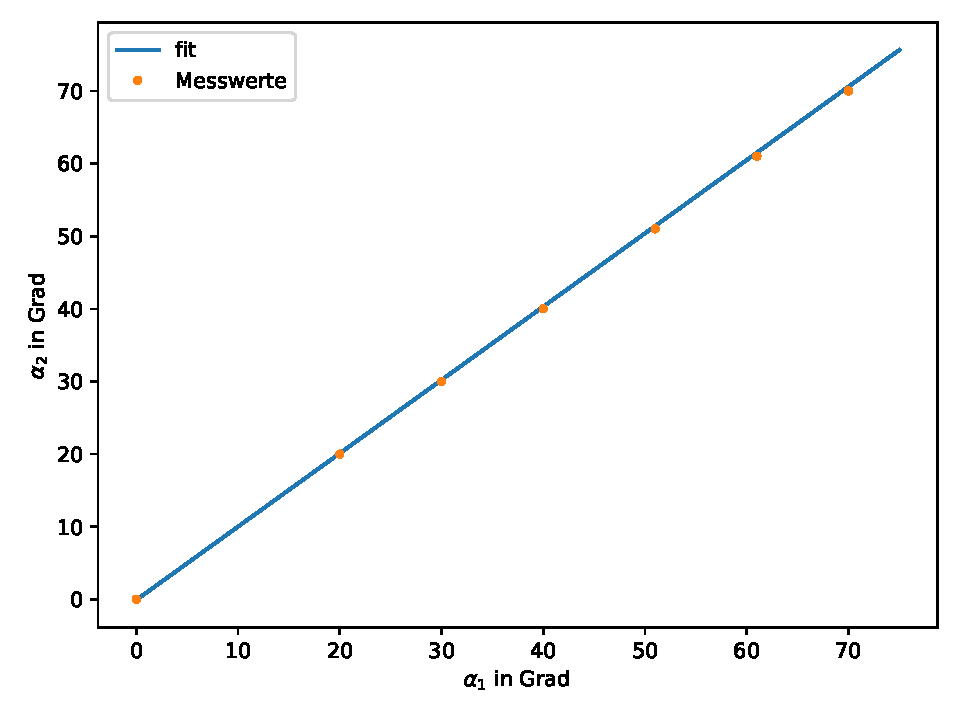
\includegraphics[width=0.7\textwidth]{build/plots/plot1.pdf}
    \caption{Die Messwerte zur für den Zerfall von $\ce{^{52}_{}V}$, inklusive Fit-Funktion halblogarithmisch dargestellt.}
    \label{img:V}
\end{figure}
\noindent
Aus dem Parameter $\mu$ lässt sich die Halbwertszeit des Isotops bestimmen. Dafür wird folgende Gleichung genutzt:
\begin{equation}
    T_{\frac{1}{2}}=\frac{\ln{2}}{\mu}
    \label{eqn:halb}
\end{equation}
Damit lässt sich nun ein Wert und aus ihm auch direkt die relative Abweichung vom Theoriewert\cite{Vanadium} bestimmen.
\begin{align*}
    T_{\frac{1}{2}V_1}&= \SI{202.61626(723460)}{\second}  \\
    T_{\frac{1}{2}\text{ theo}}&=(224.58)\si{\second} \\
    \frac{T_{\frac{1}{2}\text{ theo}}-T_{\frac{1}{2}V_1}}{T_{\frac{1}{2}\text{ theo}}}&=\SI{9.8(32)}{\percent}
\end{align*}
\newline
\noindent
Anschließend wird noch einmal ein genauerer Fit erstellt, der nur Werte nutzt, die im Zeitintervall $2\cdot T_{\frac{1}{2}V_1}$liegen.\\
Dadurch sollen die Auswirkungen der ungenauen Messungen für große $t$ minimiert werden.\\
Als Fit der selben Form, wie in Gl.\ref{eqn:fit}, ergeben sich dann folgende Parameter:
\begin{align*}
    A_{V2}&=(\SI{206.61800(944087)}{})\\
    \mu_{V2}&=\SI{0.00332(27)}{\per\second}\\\\
    T_{\frac{1}{2}V_2}&= \SI{208.92148(1674884)}{\second}\\
    \frac{T_{\frac{1}{2}\text{ theo}}-T_{\frac{1}{2}V_2}}{T_{\frac{1}{2}\text{ theo}}}&=\SI{7(7)}{\percent}
\end{align*}
Die Funktion ist auch in der Abb.\ref{img:V} zu sehen.\\\\
\noindent
Im folgenden ist die Tabelle mit den, für Abb.\ref{img:V}, genutzten logarithmierten Messwerten zu finden. 
\newpage
\begin{table}[H]
    \centering
    \small
    \begin{tabular}{S [table-format=3.1] S [table-format=1.4] S [table-format=1.4]}
        \toprule
        {$t \mathbin{\scalebox{1.5} / }\si{\second}$} &  {$\ln{N_V - N_0} $} & {$\ln{\sqrt{N_V - N_0 }}$}\\
        \midrule
        30.0                 & 5.1651& 0.0755 \\
        60.0                 & 5.2098& 0.0739 \\
        90.0                 & 4.9131& 0.0857 \\
        120.0                & 4.9772& 0.0830 \\
        150.0                & 4.9492& 0.0841 \\
        180.0                & 4.7712& 0.0920 \\
        210.0                & 4.6354& 0.0984 \\
        240.0                & 4.5333& 0.1036 \\
        270.0                & 4.3829& 0.1117 \\
        300.0                & 4.4551& 0.1077 \\
        330.0                & 4.1754& 0.1239 \\
        360.0                & 4.0086& 0.1347 \\
        390.0                & 4.2057& 0.1221 \\
        420.0                & 3.4679& 0.1765 \\
        450.0                & 3.5573& 0.1688 \\
        480.0                & 3.8516& 0.1457 \\
        510.0                & 3.7393& 0.1541 \\
        540.0                & 3.2608& 0.1958 \\
        570.0                & 3.4362& 0.1793 \\
        600.0                & 2.8943& 0.2352 \\
        630.0                & 2.5704& 0.2765 \\
        660.0                & 3.3697& 0.1854 \\
        690.0                & 3.0479& 0.2178 \\
        720.0                & 1.6236& 0.4440 \\
        750.0                & 2.6441& 0.2665 \\
        780.0                & 2.5704& 0.2765 \\
        810.0                & 3.0942& 0.2128 \\
        840.0                & 2.4043& 0.3005 \\
        870.0                & 2.7128& 0.2575 \\
        900.0                & 1.4039& 0.4955 \\
        930.0                & 1.1221& 0.5705 \\
        960.0                & 2.3097& 0.3151 \\
        990.0                & 1.9560& 0.3760 \\
        1020.0               & 2.4043& 0.3005 \\
        1050.0               & 1.9560& 0.3760 \\
        1080.0               & 2.3097& 0.3151 \\
        1110.0               & 2.4043& 0.3005 \\
        1140.0               & 1.1221& 0.5705 \\
        1170.0               & 1.8035& 0.4058 \\
        1200.0               & 1.6236& 0.4440 \\
        1230.0               & 1.8035& 0.4058 \\
        1260.0               & 1.4039& 0.4955 \\
        1290.0               & 0.7282& 0.6948 \\
        1320.0               & 1.1221& 0.5705 \\
        \bottomrule
    \end{tabular}
\caption{Die Messwerte, die in \ref{img:V} zum Ploten des halblogarithmischen Diagramms genutzt wurden.}
\label{tab:logV}
\end{table}


\subsection{Rhodium}
\begin{table}[!htbp]
    \centering
    \small
    \begin{tabular}{S [table-format=3.1] S [table-format=3.1] S [table-format=3.4] S [table-format=3.4]}
        \toprule
        {$t \mathbin{\scalebox{1.5} / }\si{\second}$} & {$N_{Rh} $} & {$N_R - \frac{1}{2}N_0 $} & {$\sqrt{N_{Rh} - \frac{1}{2}N_0 }$}\\
        \midrule
        15.0                 & 667.0                & 6.4922   & 0.0389 \\
        30.0                 & 585.0                & 6.3596   & 0.0415 \\
        45.0                 & 474.0                & 6.1464   & 0.0462 \\ 
        60.0                 & 399.0                & 5.9713   & 0.0505 \\ 
        75.0                 & 304.0                & 5.6938   & 0.0580 \\
        90.0                 & 253.0                & 5.5054   & 0.0637 \\ 
        105.0                & 213.0                & 5.3280   & 0.0696 \\ 
        120.0                & 173.0                & 5.1122   & 0.0776 \\ 
        135.0                & 152.0                & 4.9769   & 0.0830 \\ 
        150.0                & 126.0                & 4.7794   & 0.0916 \\ 
        165.0                & 111.0                & 4.6447   & 0.0980 \\ 
        180.0                & 92.0                 & 4.4430   & 0.1084 \\ 
        195.0                & 79.0                 & 4.2771   & 0.1178 \\ 
        210.0                & 74.0                 & 4.2052   & 0.1221 \\ 
        225.0                & 60.0                 & 3.9709   & 0.1373 \\ 
        240.0                & 52.0                 & 3.8074   & 0.1490 \\ 
        255.0                & 56.0                 & 3.8925   & 0.1428 \\ 
        270.0                & 53.0                 & 3.8294   & 0.1473 \\ 
        285.0                & 41.0                 & 3.5274   & 0.1714 \\ 
        300.0                & 36.0                 & 3.3685   & 0.1855 \\ 
        315.0                & 37.0                 & 3.4023   & 0.1824 \\ 
        330.0                & 32.0                 & 3.2203   & 0.1998 \\ 
        345.0                & 36.0                 & 3.3685   & 0.1855 \\ 
        360.0                & 38.0                 & 3.4351   & 0.1795 \\ 
        375.0                & 34.0                 & 3.2971   & 0.1923 \\ 
        390.0                & 40.0                 & 3.4975   & 0.1739 \\ 
        405.0                & 21.0                 & 2.6416   & 0.2669 \\ 
        420.0                & 35.0                 & 3.3334   & 0.1888 \\ 
        435.0                & 33.0                 & 3.2594   & 0.1959 \\ 
        450.0                & 36.0                 & 3.3685   & 0.1855 \\ 
        465.0                & 20.0                 & 2.5676   & 0.2769 \\ 
        480.0                & 24.0                 & 2.8353   & 0.2422 \\ 
        495.0                & 30.0                 & 3.1370   & 0.2083 \\ 
        510.0                & 30.0                 & 3.1370   & 0.2083 \\ 
        525.0                & 26.0                 & 2.9463   & 0.2292 \\ 
        540.0                & 28.0                 & 3.0462   & 0.2180 \\ 
        555.0                & 23.0                 & 2.7748   & 0.2497 \\ 
        570.0                & 20.0                 & 2.5676   & 0.2769 \\ 
        585.0                & 28.0                 & 3.0462   & 0.2180 \\ 
        600.0                & 17.0                 & 2.3061   & 0.3156 \\ 
        615.0                & 26.0                 & 2.9463   & 0.2292 \\ 
        630.0                & 19.0                 & 2.4878   & 0.2882 \\ 
        645.0                & 13.0                 & 1.7976   & 0.4070 \\ 
        660.0                & 17.0                 & 2.3061   & 0.3156 \\ 
        \bottomrule
    \end{tabular}
\caption{Die Messwerte der Zerfallraten für Rhodium mit ihren korrespondierenden Zeiten. Zusätzlich auch noch ihr $\sqrt{N}$ Fehler und die Raten abzüglich Nullraten.}
\label{tab:Rh}
\end{table}



Für die Messwerttabelle \ref{tab:Rh} von $\ce{^{104}_{}Rh}$ und $\ce{^{104i}_{}Rh}$ wurde von den Zählraten die Hälfte des oben berechneten Wertes der Nullrate genutzt, 
da für diesen Versuch die Messwerte in einem Intervall von $\increment t=15 \si{\second}$ aufgenommen wurden, und nicht wie zuvor $\increment t=30\si{\second}$.\\
In diesem Auswertungsteil wird, da sich die beiden Zerfälle für kleine Zeiten überlagern, erst der mit der größeren Halbwertszeit untersucht um durch Extrapolation seiner Zerfälle
die des kurzlebigeren Isotops zu untersuchen.\\\\
\noindent
Die Messwerte dieses Zerfalles bestehen aus der Überlagerung zwei unterschiedlicher Zerfälle. Bei der Auswertung müssen diese also möglichst unabhängig voneinander untersucht werden.
Für die Untersuchung wird dafür grafisch abgeschätzt ab welchem Punkt der Zerfall des kurzlebigeren Isotops $\ce{^{104}_{}Rh}$ an Bedeutung verliert. 
Dafür wurde ein Wert von $t' =\SI{250}{\second} $ abgeschätzt.\\
Im Folgenden wurde aber sicherheitshalber erst, zur Bestimmung der Halbwertszeit von $\ce{^{104i}_{}Rh}$, Werte ab  $t' =\SI{300}{\second} $, genutzt.\\
Die Messwerte und die Aufteilung in zwei Intervalle sind in der folgenden Abbildung, Abb.\ref{img:Rh1}, noch einmal grafisch veranschaulicht.
Dort sind auch die Fit-Funktionen der beiden Halbwertszeiten, sowie ihre Kombination aufgetragen.\\
Die Kombinationsfunktion hat dabei folgende Form, wobei die Parameter erst noch bestimmt werden müssen:
\begin{equation*}
    f_\text{Kombi}(t)= A_{Rh1} \symup{e}^{-\mu_{Rh1} t} + A_{Rh2} \symup{e}^{-\mu_{Rh2} t} 
\end{equation*}



\begin{figure}[H]
    \centering
    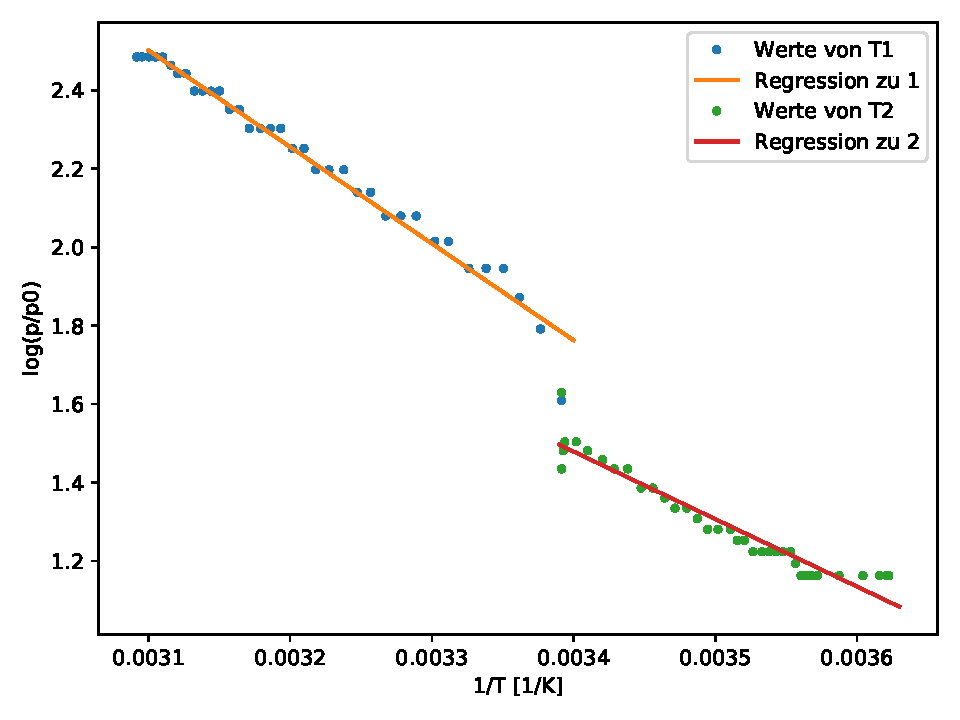
\includegraphics[width=0.70\textwidth]{build/plots/plot2.pdf}
    \caption{Die Messwerte zur für den Zerfall von $\ce{^{104}_{}Rh}$ und $\ce{^{104i}_{}Rh}$ halblogarithmisch dargestellt. 
    Zusätzlich auch noch die Fit-Funktionen für beide Isotope einzeln und kombiniert. Außerdem auch noch der Punkt ab dem ein Abflachen des ersten Zerfalls zu beobachten ist.}
    \label{img:Rh1}
\end{figure}
\noindent
\noindent
Für die Erstellung dieser Grafik wurden die logarithmierten Messwerte, die in der Tabelle\ref{tab:logRh} zu finden sind, genutzt.

\begin{table}[H]
    \centering
    \begin{tabular}{S [table-format=3.1] S [table-format=1.4] S [table-format=1.4]}
        \toprule
        {$t \mathbin{\scalebox{1.5} / }\si{\second}$} &  {$\ln{N_{Rh} - N_0} $} & {$\ln{\sqrt{N_{Rh} - N_0 }}$}\\
        \midrule
        15.0                 & 6.4922  & 0.0389  \\
        30.0                 & 6.3596  & 0.0415  \\
        45.0                 & 6.1464  & 0.0462  \\
        60.0                 & 5.9713  & 0.0505  \\
        75.0                 & 5.6938  & 0.0580  \\
        90.0                 & 5.5054  & 0.0637  \\
        105.0                & 5.3280  & 0.0696  \\
        120.0                & 5.1122  & 0.0776  \\
        135.0                & 4.9769  & 0.0830  \\
        150.0                & 4.7794  & 0.0916  \\
        165.0                & 4.6447  & 0.0980  \\
        180.0                & 4.4430  & 0.1084  \\
        195.0                & 4.2771  & 0.1178  \\
        210.0                & 4.2052  & 0.1221  \\
        225.0                & 3.9709  & 0.1373  \\
        240.0                & 3.8074  & 0.1490  \\
        255.0                & 3.8925  & 0.1428  \\
        270.0                & 3.8294  & 0.1473  \\
        285.0                & 3.5274  & 0.1714  \\
        300.0                & 3.3685  & 0.1855  \\
        315.0                & 3.4023  & 0.1824  \\
        330.0                & 3.2203  & 0.1998  \\
        345.0                & 3.3685  & 0.1855  \\
        360.0                & 3.4351  & 0.1795  \\
        375.0                & 3.2971  & 0.1923  \\
        390.0                & 3.4975  & 0.1739  \\
        405.0                & 2.6416  & 0.2669  \\
        420.0                & 3.3334  & 0.1888  \\
        435.0                & 3.2594  & 0.1959  \\
        450.0                & 3.3685  & 0.1855  \\
        465.0                & 2.5676  & 0.2769  \\
        480.0                & 2.8353  & 0.2422  \\
        495.0                & 3.1370  & 0.2083  \\
        510.0                & 3.1370  & 0.2083  \\
        525.0                & 2.9463  & 0.2292  \\
        540.0                & 3.0462  & 0.2180  \\
        555.0                & 2.7748  & 0.2497  \\
        570.0                & 2.5676  & 0.2769  \\
        585.0                & 3.0462  & 0.2180  \\
        600.0                & 2.3061  & 0.3156  \\
        615.0                & 2.9463  & 0.2292  \\
        630.0                & 2.4878  & 0.2882  \\
        645.0                & 1.7976  & 0.4070  \\
        660.0                & 2.3061  & 0.3156  \\
        \bottomrule
    \end{tabular}
\caption{Die Messwerte, die in \ref{img:Rh1} zum Ploten des halblogarithmischen Diagramms genutzt wurden.}
\label{tab:logRh}
\end{table}
\noindent

\subsubsection{Halbwertszeit von $\ce{^{\text{104i}}_{}\text{Rh}}$}

\noindent
Nun wird für das zuvor beschriebene Intervall ein Fit auf die Messwerte bestimmt. 
Dafür wird die Funktion aus \ref{eqn:fit} genutzt.\\
Die Werte ergeben sich dann zu:
\begin{align*}
    A_{Rh1}&=(\SI{72.29855(1606114)}{})\\
    \mu_{Rh1}&=\SI{0.00264(000050)}{\per\second}
\end{align*}
Hieraus lassen sich die Werte für die Halbwertszeit, mit Gl.\ref{eqn:halb}, und die die relative Abweichung vom Theoriewert\cite{Rhodium} bestimmen.
\begin{align*}
    T_{\frac{1}{2}\ce{^{104i}_{}Rh}}&= \SI{262.38900(4969076)}{\second}\\
    T_{\frac{1}{2}\ce{^{104i}_{}Rh}\text{ theo}}&= \SI{260.4}{\second}\\
    \frac{T_{\frac{1}{2}\ce{^{104i}_{}Rh} \text{ theo}} - T_{\frac{1}{2}\ce{^{104i}_{}Rh}}}{T_{\frac{1}{2}\ce{^{104i}_{}Rh}\text{ theo}}}&=\SI{-01(19)}{\percent}
\end{align*}

\subsubsection{Halbwertszeit von $\ce{^{\text{104}}_{}\text{Rh}}$}

In diesem Abschnitt wird für das Zeitintervall kleiner als $t'$ eine Bestimmung der Halbwertszeit von $\ce{^{104}_{}Rh}$ vorgenommen.\\
Dafür wird ein nochmal kleineres Intervall gewählt, in dem die Einflüsse des langlebigeren Zerfalls wesentlich kleiner sind als die des kurzlebigeren.
Für dieses Intervall werden dann mit Hilfe des Fits extrapolierte Zählraten errechnet, die dann von den tatsächlich gemessenen Raten abgezogen werden.\\
Diese neu errechneten Werte, inklusiver der Werte, die zum Zeichnen des Plots genutzt wurden, findet man in der folgenden Tabelle \ref{tab:Rh2}.\\
Mit diesen Werten wird anschließend auch der Fit erstellt.\\

\begin{table}[H]
    \centering
    \begin{tabular}{S [table-format=3.3] S [table-format=3.3] S [table-format=2.3] S [table-format=1.3] S [table-format=1.3]}
        \toprule
        {$t \mathbin{\scalebox{1.5} / }\si{\second}$} &{$N_{Rh} - f_{Rh}(t) $} & {$\sqrt{N_{Rh2} - f_{Rh}(t) }$}&  {$\ln{N_{Rh2} - f_{Rh}(t)} $} & {$\ln{\sqrt{N_{Rh2} - f_{Rh} }}$}\\
        \midrule
        15.000 & 591.779 & 16.720 & 6.383 & 0.028  \\  
        30.000 & 506.739 & 17.425 & 6.228 & 0.034  \\
        45.000 & 392.575 & 18.181 & 5.973 & 0.046  \\
        60.000 & 314.284 & 18.991 & 5.750 & 0.060  \\
        75.000 & 215.860 & 19.858 & 5.375 & 0.092  \\
        90.000 & 161.297 & 20.786 & 5.083 & 0.129  \\
        105.000 & 117.590 & 21.780 & 4.767 & 0.185  \\
        120.000 & 73.734 & 22.843 & 4.300 & 0.310  \\
        135.000 & 48.721 & 23.980 & 3.886 & 0.492  \\
        \bottomrule
    \end{tabular}
\caption{Die Messwerte, die in \ref{img:Rh2} zum Ploten des halblogarithmischen Diagramms genutzt wurden. Es sind die Messwerte für dieses Intervall abzüglich der Funktionswerte des ersten Fits.}
\label{tab:Rh2}
\end{table}
\noindent
Hiermit lässt sich eine Fit Funktion erstellen, die relativ unabhängig vom Zerfall von $\ce{^{104i}_{}Rh}$ ist.
Dafür wird wieder eine $\symup{e}$-Funktion der Form der Gleichung \ref{eqn:fit} genutzt.\\
Dies führt zu den Werten:
\begin{align*}
    A_{Rh2}&=(\SI{812.20494(3787690)}{})\\
    \mu_{Rh2}&=\SI{0.01747(000107 )}{\per\second}
\end{align*}
Für dieses Intervall ist lässt sich dies wie folgend grafisch darstellen.
\begin{figure}[H]
    \centering
    \includegraphics[width=0.65\textwidth]{build/plots/plot3.pdf}
    \caption{Das Intervall, welches für die Untersuchung des kurzlebigeren Isotops genutzt wurde, inklusive Fit-Funktion.}
    \label{img:Rh2}
\end{figure}

\noindent
Wie zuvor lassen sich aus dem zuvor bestimmten $\mu_{Rh2}$ direkt die Werte für die Halbwertszeit und die die relative Abweichung vom Theoriewert\cite{Rhodium} bestimmen.
\begin{align*}
    T_{\frac{1}{2}\ce{^{104}_{}Rh}}&= \SI{39.68759(243149)}{\second}\\
    T_{\frac{1}{2}\ce{^{104}_{}Rh}\text{ theo}}&= \SI{42.3}{\second}\\
    \frac{T_{\frac{1}{2}\ce{^{104}_{}Rh} \text{ theo}} - T_{\frac{1}{2}\ce{^{104}_{}Rh}}}{T_{\frac{1}{2}\ce{^{104}_{}Rh}\text{ theo}}}&=\SI{6(6)}{\percent}
\end{align*}
